\section{Evaluation}
\label{sec:eval}

\subsection{Setup}
We perform the evaluation based on the most up-to-date version of Wasm
standard, Wasm 2.0. We have crafted \specdsl, which is the description of the
syntax, validation, and execution semantics of Wasm 2.0, written in DSL.
which plays the role of the initial input of SpecTec framework.
In order to focus on the core of the Wasm 2.0 semantics,  we made
the deliberate choice to omit the SIMD instructions. We also omitted the
auxiliary functions for numeric instructions, mainly related to the bit level
manipulation of Wasm values. Instead of writing these numeric functions in DSL,
we decided to borrow the implementations from the reference interpreter.
In addition, some rules or auxiliary helper functions are specified in
different way in \specdsl compared to the official specification.  For
example, the current standard of Wasm 2.0 uses the evaluation context to
describe the behavior of `br` and `return` instructions, so that multiple block
contexts can be popped at once. Instead, we use \textit{bubble-up style} for
describing the rules for these instructions, which escape one context at
applying one reduction rule. Also, the auxiliary functions for instantiation
of modules, \textit{instantiate}, are rewritten in a way that avoid the cyclic
bindings within premises. We have confirmed that our rewritten rules are
equivalent to original rules by the Wasm spec developers.  The overall Lines of
Code (LoC) for the entire \specdsl amounted \inred{1,147}. This represents a
significant reduction compared to the ten thousand of LoC present in the
ReStructuredText document for actual specification.

In the subsequent sections, we will showcase the capabilities of SpecTec in the following aspects:
1) Generation of two artefacts: LaTeX and Prose specification
2) Meta-level execution of Wasm test suite
3) Ability to detect and prevent spec errors
4) Generality towards new proposals.

\subsection{Generation of LaTeX and Prose Specification}:
The \specdsl was successfully transformed into LaTeX, including all of syntax,
validation, and execution semantics.  Also, the prose for the execution
semantics was successfully generated.  This includes the prose for both of each
reduction rules of Wasm instructions, and the module instantiation functions.
The automatically generated PDF document, including both formal and prose
notations, is available as the supplementary material[?].  The result indicates
the capability of SpecTec to generate formal notation specifications from DSL
representations, contributing to the ease of documentation.

\subsection{Meta-level execution of Wasm Test Suite}
In this section we illustrate the result of interpreting official Wasm test suite[?]
with our meta-level Wasm interpreter.  This evaluation serves dual purposes: 1) It
demonstrates the ability of the meta-level interpreter to interpret the actual,
real-world Wasm program, and 2) It provides assurance regarding the correctness of
all of the \specdsl we crafted, the translation process of \specdsl into \al,
and the resulting generated prose specification.

The official test of Wasm is written in `.wast' format[?], which is a scripting
language designed for testing Wasm implementations.  A `.wast' file consists of
one or more Wasm modules, and a sequence of assertions that verify if the actual
behavior matches the expected behavior.  Among seven kinds of assertions, we
exclude three kinds of assertions that are related to parsing and validation
phase of Wasm, which we currently do not support.  Also, we exclude one more
kind of assertion that is designed to test if an invocation of Wasm function
results in an infinite loop.  As a result, we target three kinds of assertions:
\textit{AssertUninstantiable} which tests if a module instantiation results in
a Trap, \textit{AssertTrap} which tests if a function invocations results in a
Trap, and \textit{AssertReturn} which tests if a function invocation returns a
expected value.

There were 90 test scripts, comprising \inred{21,363} AssertReturn,
\inred{2,354} AssertTrap, and \inred{34} AssertUninstantiable.  The entire test
suite took \inred{???} seconds to run. Remarkably, the test pass rate was
100\%. Every target assertion passed, indicating that every module instantiation
and function invocation exhibited the expected behaviors.  This result
highlights two key points: firstly, SpecTec is indeed capable of effectively
executing real-world Wasm programs. Secondly, the specification we manually
crafted in DSL, and the process that translates DSL into \al, are both correct.

\subsection{Detecting and Preventing Errors}
To assess the effectiveness of SpecTec in preventing human errors in
documenting the specification, we conducted an in-depth investigation into
actual errors that had previously occurred in the main branch of the repository
for Wasm standard~\cite{wasmspecrepo}. Our objective was to determine whether
SpecTec could have prevented these errors. We classified the investigated
errors into four distinct categories.

\begin{figure}
  \centering
  \begin{subfigure}[b]{0.49\textwidth}
    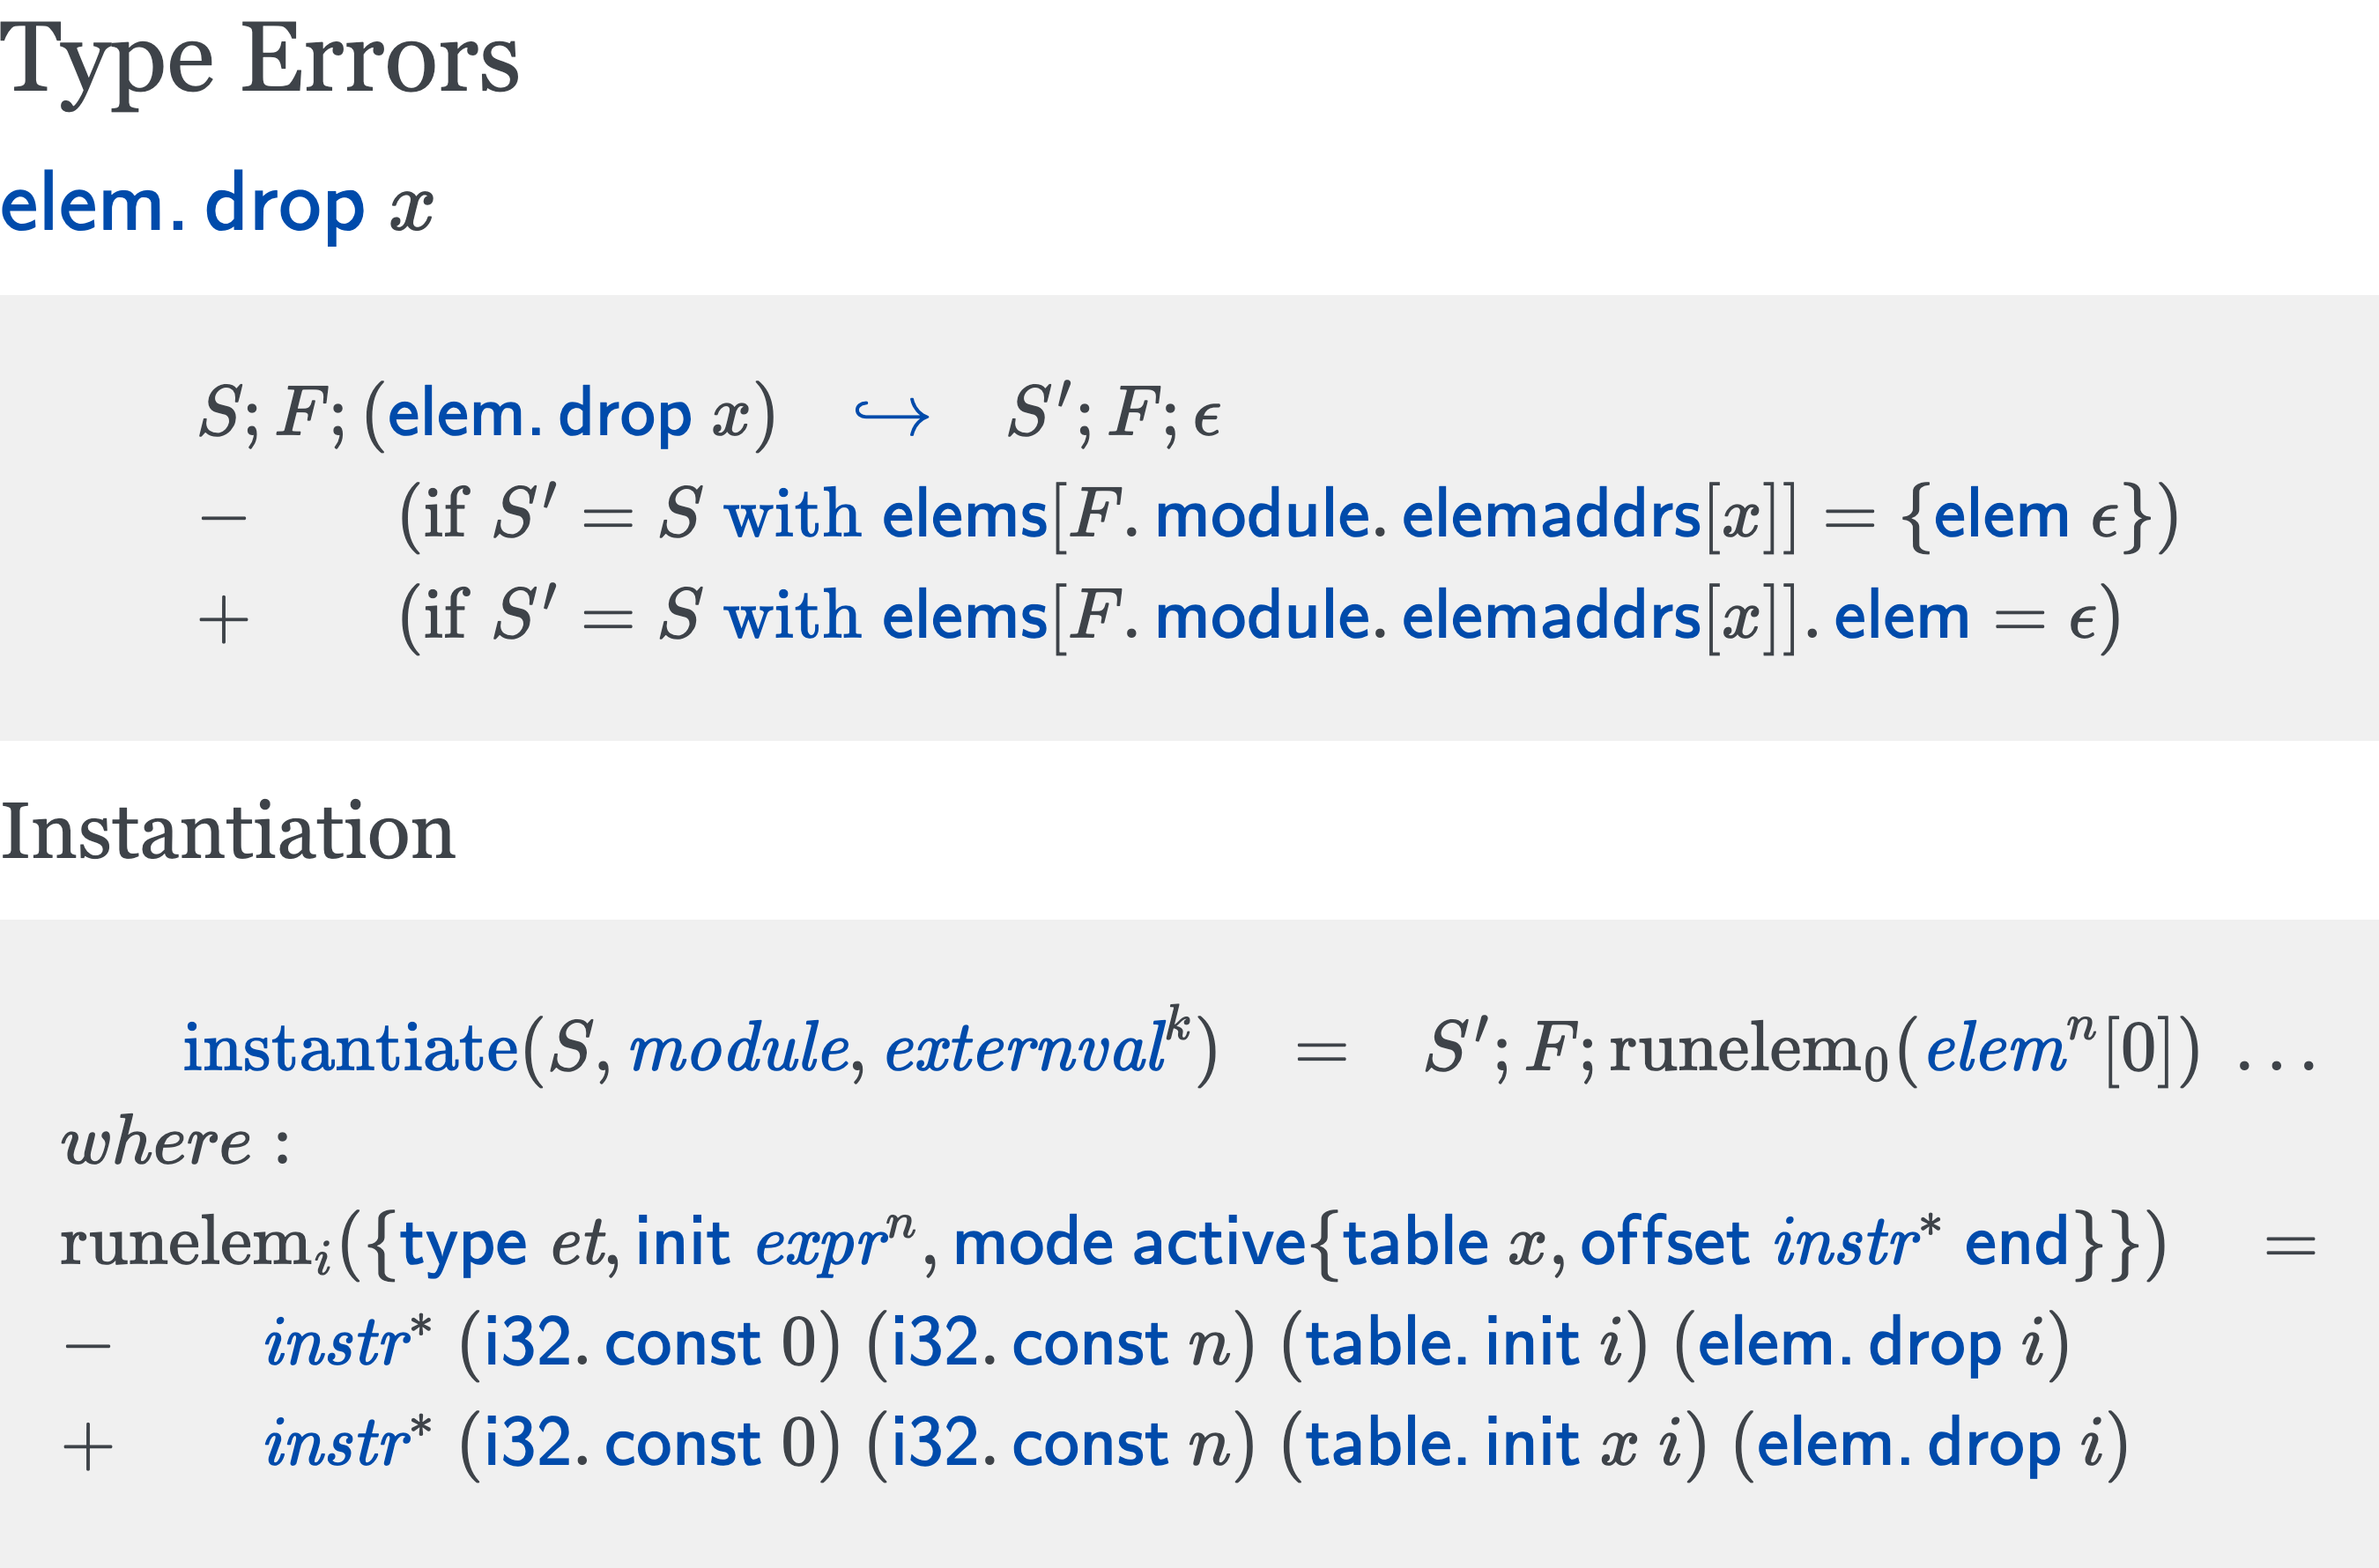
\includegraphics[width=\textwidth]{../img/type-error}
    \caption{Type Error}
    \label{fig:type-error}
  \end{subfigure}
  \begin{subfigure}[b]{0.49\textwidth}
    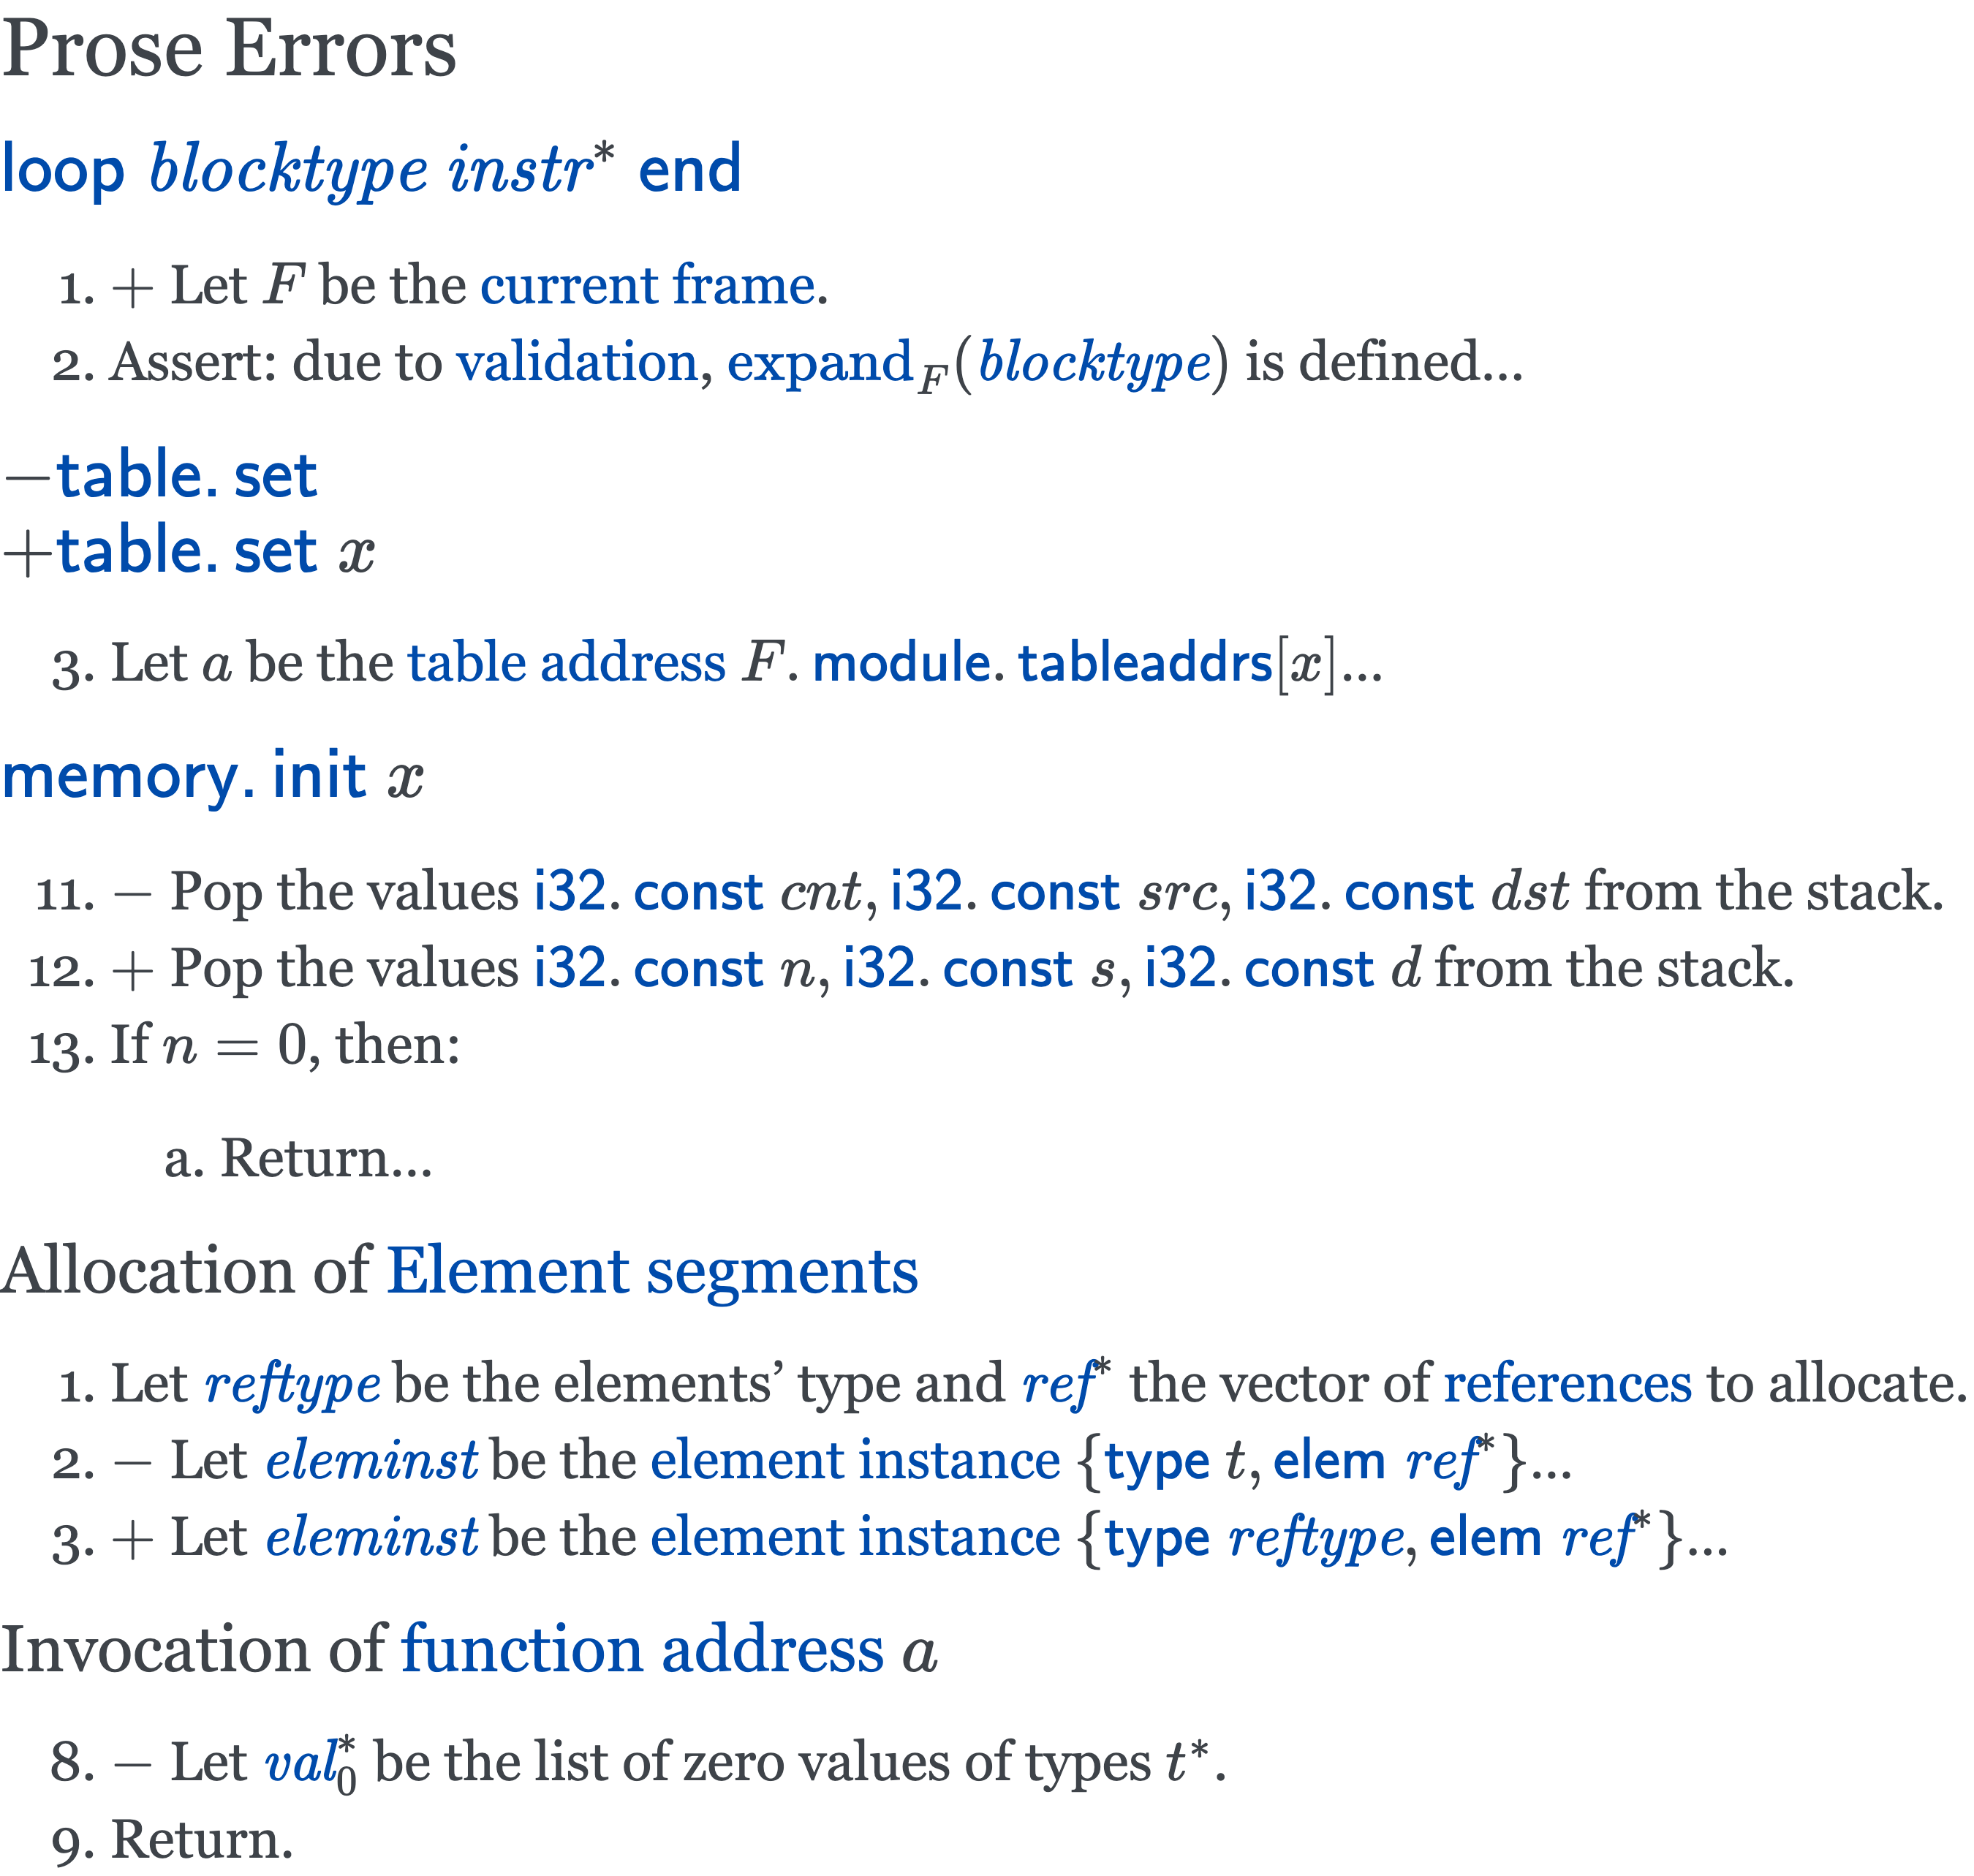
\includegraphics[width=\textwidth]{../img/prose-error}
    \caption{Prose Error}
    \label{fig:prose-error}
  \end{subfigure}
  \begin{subfigure}[b]{0.49\textwidth}
    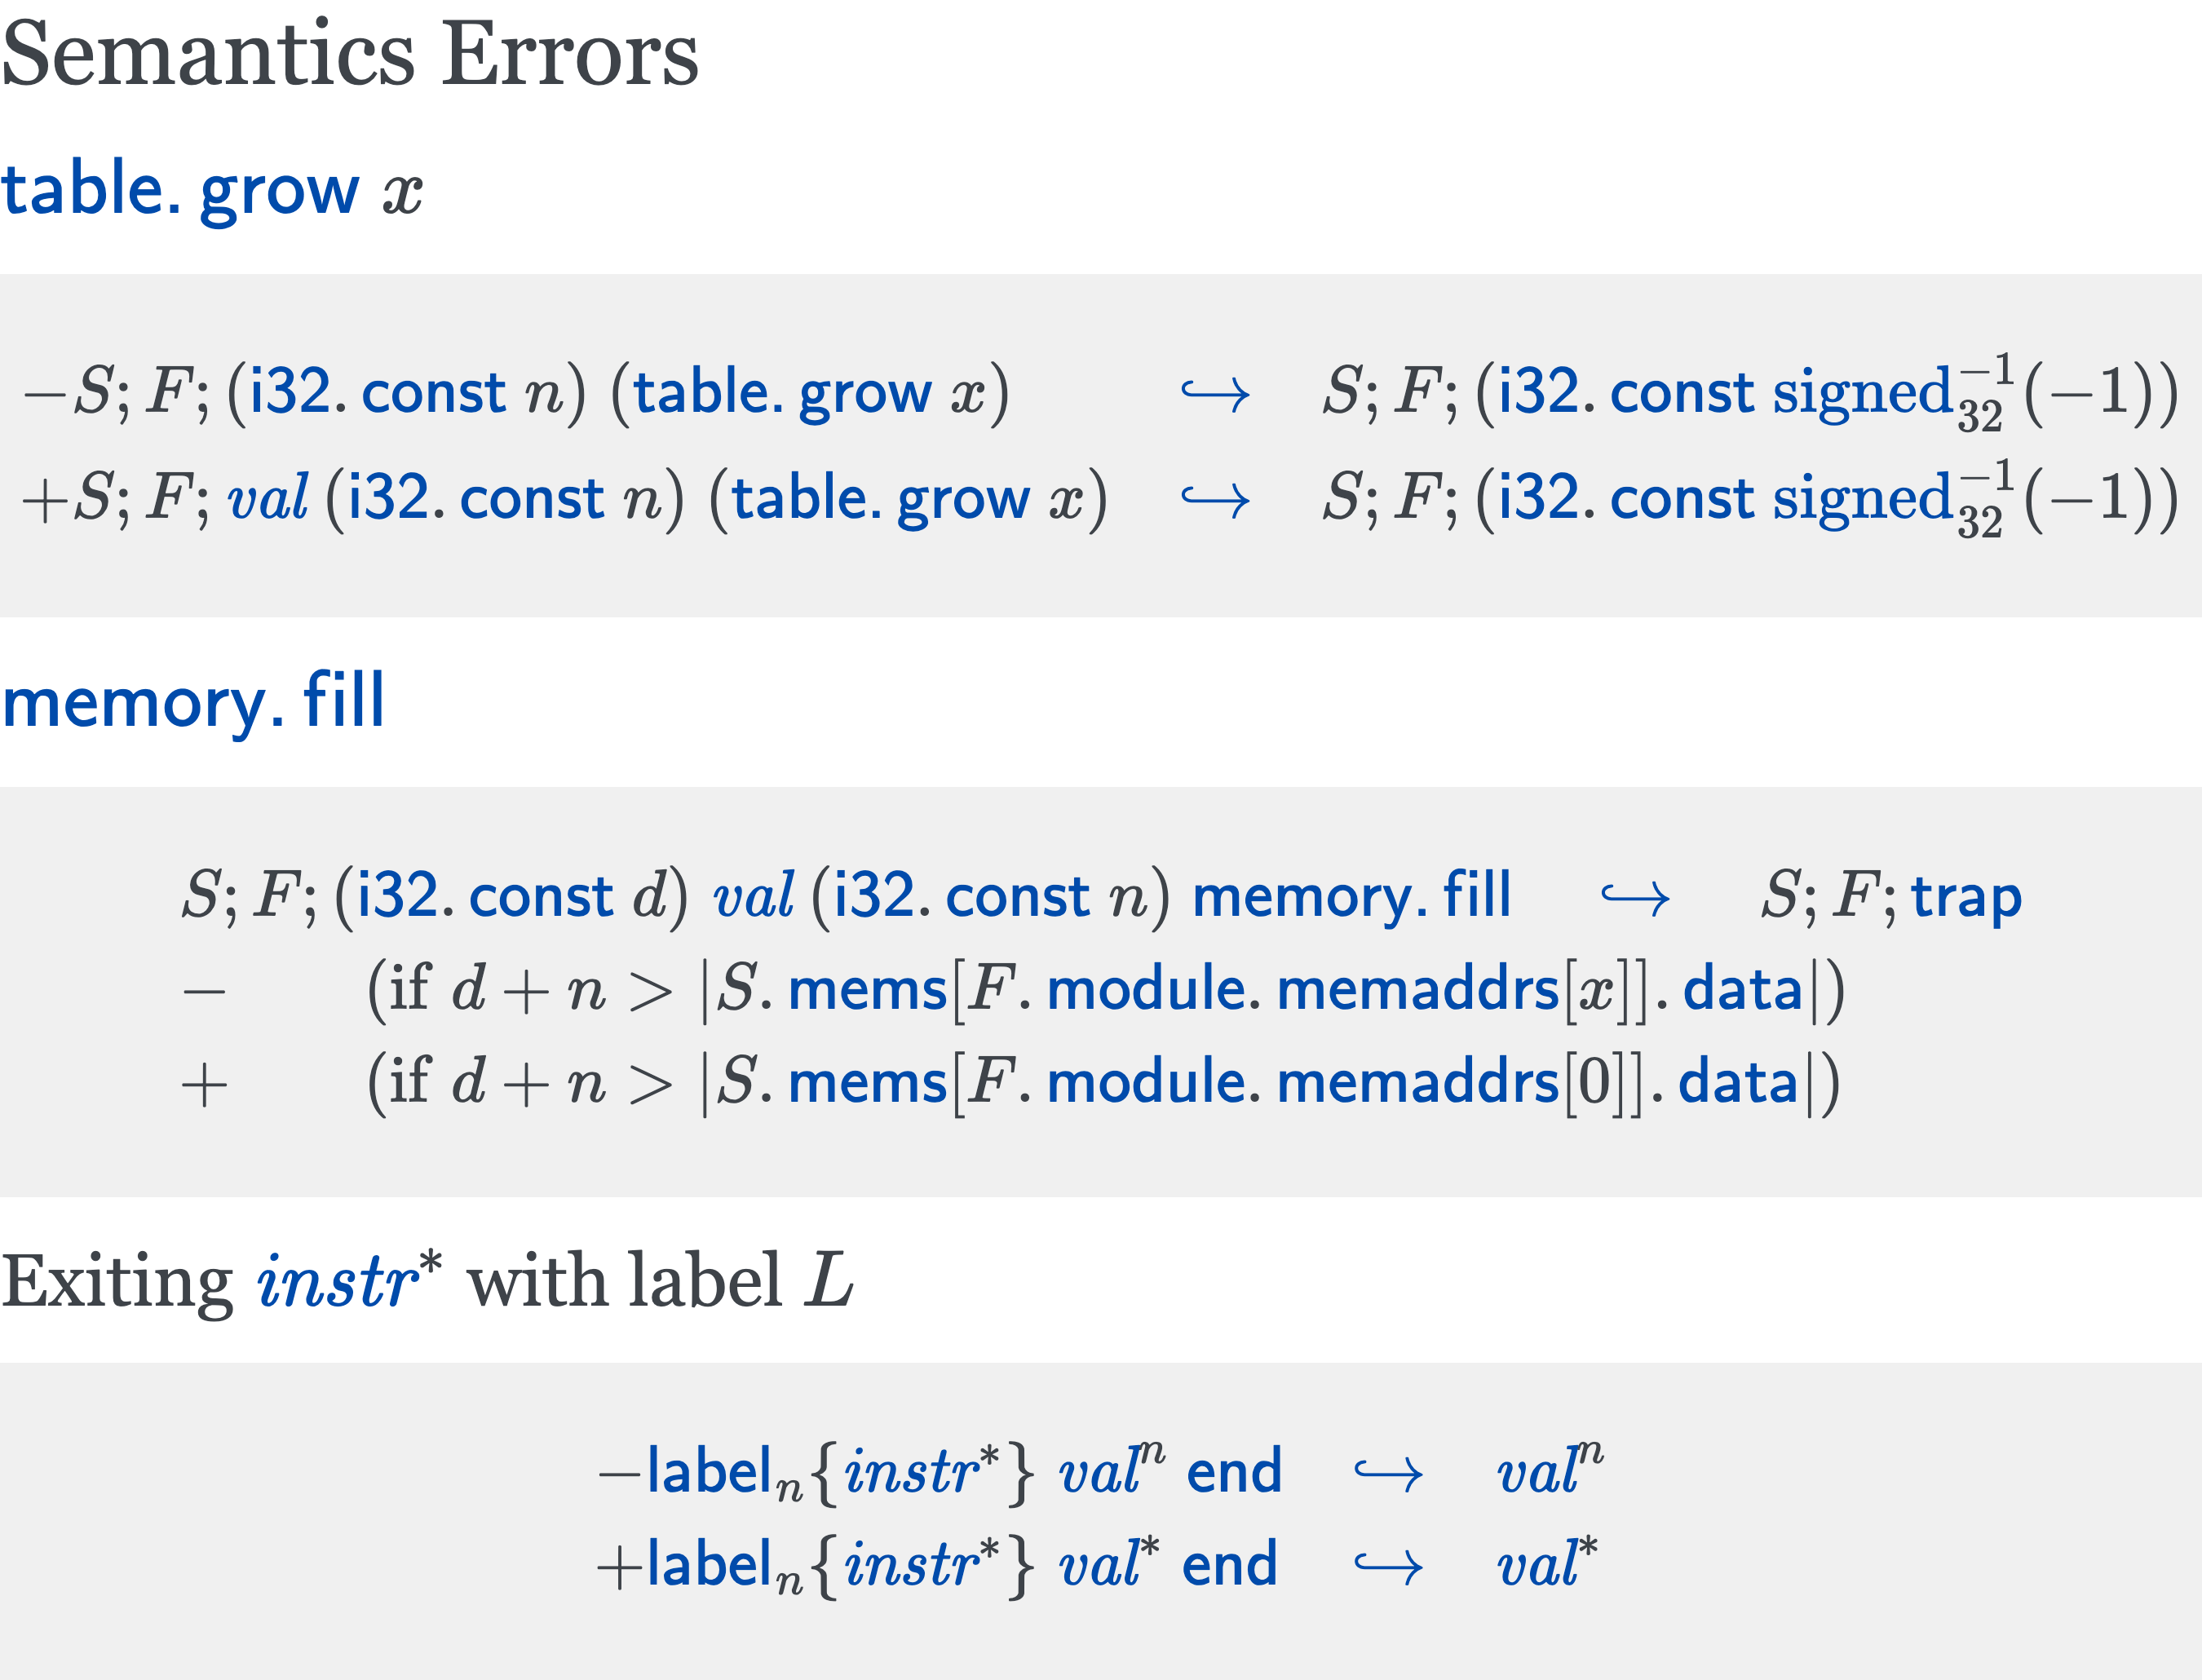
\includegraphics[width=\textwidth]{../img/semantics-error}
    \caption{Semantics Error}
    \label{fig:semantics-error}
  \end{subfigure}
  \caption{The list of errors in Wasm specification that could have been detected / prevented by SpecTec}
\end{figure}

\textbf{Type Errors}
This category represents the spec errors that could have been prevented by the
type checker of SpecTec. There were two errors in this category, as illustrated
in Fig.~\ref{fig:type-error}. These instances included an omission of the field
\textit{TYPE} during the initialization of the element instance in the
\textit{elem.drop} execution semantics, an arity mismatch for the Wasm
instruction \textit{table.init} during module instantiation.  We artificially injected each of these
errors into the \specdsl and applied type checker of SpecTec.  Subsequently, we
figured out that SpecTec successfully identified and reported the Type Errors.
The error message gives the information about the exact location of the error
within the specification, and the exact reason for the error.  This result
signifies its capability to detect mistakes made by spec writers, and aid
fixing it.

\textbf{Prose Errors}
This category represents errors in the prose that could have been prevented by
automatic prose generation from the first place. There were five errors in this
category as illustrated in Fig.~\ref{fig:prose-error}. These five errors
encompassed mainly about the free identifier issues, and an outdated step that
introduced a new variable \textit{val\_0} which was never utilized during
function invocation. Our automatic prose generation process
is free from these types of errors due to the nature of automatic generation,
and we verified that the corresponding prose was generated accurately, devoid
of any such issues.

\textbf{Semantics Errors}
This category represents semantics errors within semantics that incurs the
incorrect behavior of Wasm, which could have been prevented by the meta-level
interpretation with SpecTec.  There were three errors in this category as
illustrated in Fig.~\ref{fig:semantics-error}. These include missing a value in
the value stack of a reduction rule of \textit{table.grow}, using a wrong
memory index for \textit{memory.fill} (and \textit{memory.init}), or popping a
wrong number of values when exiting from a \textit{label}.   We manually injected these
errors into the \specdsl, and subsequently executed the official tests against them
using our indirect interpreter. In all cases, the corresponding tests resulted
in a failure as expected, indicating that our indirect interpreter was proficient
in detecting these errors.

\textbf{Editorial Fixes}
In addition to the specification errors that directly impacts its behavior, we
also identified numerous editorial fixes that addresses the presentational
issues such as typographical errors in LaTeX or inconsistency in writing style
within the document. Once again, SpecTec can effectively address these types of
issues because because it ensures that the generated specifications adhere to a
predefined structure and style, eliminating the likelihood of manual errors or
inconsistencies.

These emperical results demonstrate that SpecTec is effective at preventing a
wide range of human errors within the WebAssembly specification.  Its
capabilities extend to detecting and addressing type errors, prose errors,
semantics errors, as well as editorial fixes. This is a strong evidence that
leveraging SpecTec can significantly enhance the robustness and reliability of
the specification writing process.

\subsection{Generality}
In this section, we present the generality of SpecTec, by applying it to five
%WebAssembly proposals currently at or about to enter phase 4 at the time of
WebAssembly proposals that are about to be officially standardized in Wasm at
the time of writing. These proposals include Tail Call[?], Extended Constant
Expressions[?], Typed Function References[?], Garbage Collection[?], and
Multiple Memories[?].

First, we extended the DSL-spec for each of these proposals. Each
of the five proposals was successfully described using DSL.  Despite the fact
that the new proposals were not heavily considered during the initial design
process of SpecTec, the required modifications in SpecTec were minimal,
primarily involving the addition of new custom operators for notations specific
to some of proposals. This demonstrates the versatility and adaptability of
SpecTec in effectively expressing the semantics of diverse Wasm features.

Next, we used SpecTec to automatically generate both LaTeX and Prose
specifications.  All proposals were successfully transformed into LaTeX format,
mainly thanks to the clever design of DSL.  Out of the 34 Wasm instructions
that are either newly introduced or modified by the proposals, all but two had
their semantics correctly translated into \al, and subsequently into prose. For
the two Wasm instructions with incorrect translations, \inred{we revised the
corresponding reduction rules to be compatible with the DSL-to-AL translator,
albeit making the reduction rules slightly less concise.} Our objective is to
enhance the translator's capability to handle more concise reduction rules in
the future. The proposal also introduced dozens of new auxiliary helper
functions, all of which were translated without any issues.  These results
affirm the robustness of LaTeX and prose generation against the introduced
proposals.

Following the generation of \al, we conducted testing using the tests of
proposals against the generated \al.  The only component we needed to borrow
from the reference interpreter was the calculation of subtyping of Wasm types,
introduced by Garbage Collection proposal. This was necessary because the
subtyping rules of Wasm is located in the validation section of specification,
which we have not yet extract into an executable algorithm yet.  Given this
consideration, the interpretation was successful: the indirect interpreter was
able to instantiate the Wasm modules in the tests and invoke the Wasm functions
of assertions.  The pass rate achieved was again 100\%.  This confirms that the
meta-level interpreter we have developed can be extended to handle the new
proposals, indicating the potential of our approach in providing assurance
regarding the correctness of the semantics of new Wasm features.

Furthermore, during the comparison of the artifacts generated by SpecTec with
the actual proposals, we identified certain discrepancies. Upon closer
examination, we found that these disparities arose from errors within the
official proposals themselves, encompassing both formal and prose notations. In
total, we identified and reported \inred{nine} such errors to the specification
writer, all of which were subsequently rectified.  This discovery emphasizes
that SpecTec's capacity to produce more reliable artifacts is not limited to
the current version of Wasm, but extends to future proposals as well.

Overall, the evaluation results indicate that the SpecTec approach is highly
generalizable and adaptable. It successfully accommodates a range of Wasm
proposals, accurately capturing their semantics in both formal and prose
notations. The minimal manual intervention required further underscores the
efficiency and reliability of SpecTec.  In addition, the demonstrated
capability of SpecTec to interpret the tests and identify errors of actual
proposals further supports its generality.  These findings affirm the
potential of SpecTec as a effective tool for streamlining the specification
process, not only for the current state of WebAssembly but also for
accommodating future advancements and extensions in the language.

%\subsection{Others}
%\begin{itemize}
%\item anecdotal evidence
%\begin{itemize}
%\item no need to write prose
%\item code review: readability
%\end{itemize}
%
%\item qualitative evaluation?
%\begin{itemize}
%\item compactness of writing? LoC?
%\item arity issues?
%\end{itemize}
%
%\item more quantitative evaluation
%\begin{itemize}
%\item coverage of the prose/LaTeX specification
%\end{itemize}
%\end{itemize}
